\documentclass[14pt]{extreport}
\usepackage[utf8]{inputenc}
\usepackage[german]{babel}
\usepackage{longtable}
\usepackage{wrapfig}
\usepackage{graphicx}
\usepackage{biblatex}
\usepackage{amssymb}
\usepackage{longtable}
\addbibresource{kvmVsEsxi.bib}

\author{Dane Wicki}
\title{KVM on Z vs. ESXi}

\begin{document}
\maketitle

\begin{abstract}
Virtualisierung hat seinen Ursprung schon in den Frühen 1960er Jahren, als die Computersysteme noch gross und teuer zu warten waren. Der Ursprung findet sich bei den Mainframes, eine Plattform, welche auch heute noch in Gebrauch ist, obschon sie tot geglaubt wurde. IBM entwickelte die Virtualisierung, damit die User die Computer Ressourcen untereinander teilen konnten, und diese Trotzdem noch parallel gebraucht werden konnten. Heutzutage erfreut sich die Virtualisierung eines enormen Hypes, welcher zu vielen verschiedenen Softwarelösungen geführt hat.

Die Virtualisierung ermöglicht das ausführen mehreren Virtuellen Maschinen, welche auf einem einzigen Host laufen. Diese Arbeit soll nun einen Vergleich zweier moderner Virtualisierungslösungen aufzeigen. KVM on Z ist die Erste Lösung, auf welche eingegangen werden wird. Es ist eine Opensource Lösung, welche in den Linux Kernel integriert wurde. 
ESXi, die 2. Lösung, ist eine Weitere Möglichkeit um zu Virtualisieren. Diese Lösung wird von VMWare vertrieben und ist nicht ganz so Quelloffen wie seine zu gegenüberstellende Lösung.

\end{abstract}

\tableofcontents

\chapter{Einleitung}
TODO
\chapter{Grundlagen}
\section{Grundlagen der Virtualisierung}
Virtuell ist laut Duden etwas, was nicht echt, nicht in der Wirklichkeit vorhanden, also nur scheinbar vorhanden ist. Wenn wir nun von einer Virtualisierung sprechen im Bereich der IT hat dies viel mit dieser Definition zu tun. Wenn wir nun eine Betriebssystem Instanz auf einem nicht vorhanden, also virtuellen Rechner installieren, nennen wir das Virtualisierung. Aber was meine ich nun mit dem virtuellen Rechner und wie kann ich darauf etwas laufen lassen wenn er doch nicht existiert?\\
\\
Nehmen wir doch mal an ich habe einen nicht Virtuellen Rechner, also einen wirklich vorhanden rechner vor mir. Nun Installiere ich das Betriebssystem auf eben jenem Rechner, so habe ich einen uns gewohnten Rechner. Nun könnte ich jedoch auf diesem Rechner eine Software laufen lassen, die einen weiteren Rechner herstellt, also einer, welcher nicht wirklich vorhanden ist, nur scheinbar vorhanden ist, so ist dieser Rechner virtuell. Und wie auf einem vorhandenen Rechner, kann ich auf diesem virtuellen Rechner eine Betriebssystem Instanz installieren, so habe ich einen Virtuellen Rechner.\\
\\
Also versteht man unter der Informatik unter dem Begriff Virtualisierung unter anderem die Technologie, bei welcher das Betriebssystem nicht unmittelbar auf einer physischen Instanz, einem physisch vorhanden Rechner installiert ist, sondern auf der Hardware über einer Zwischenschicht. Diese Zwischenschicht abstrahiert die reale physische Hardware, ist also nicht wirklich vorhanden. Die auf dieser Zwischenschicht laufende Betriebssystem Instanz wird als Gastsystem bezeichnet. \\
\\
Auf der realen physikalischen Hardware muss jedoch auch eine Software laufen, welche diese virtuellen Systeme erstellt, diese Software wird als Hypervisor bezeichnet. Der Hypervisor dient in erster Linie der Verwaltung und Zuteilung der Ressourcen für die einzelnen Gastsysteme. Dabei soll der Hypervisor die Ressourcen so verteilen, dass das Gastsystem die Ressourcen zur Verfügung gestellt bekommt, wenn es diese auch benötigt.\\
\\
Dank der Virtualisierung lassen sich also mehrere Gastsysteme auf einem einzelnen Hypervisor zum Laufen zu bringen. Diese Gastsystem sind zudem nicht direkt abhängig von der bestehenden Hardware, so dass es auch möglich ist, dasselbe Gastsystem auf mehreren verschiedenen physikalischen Rechner zum Laufen zu bringen sofern der Hypervisor auf dieser neuen physikalischen Instanz zum Laufen gebracht werden kann. Dies bringt den Enormen Vorteil, dass ein virtualisiertes Betriebssystem auf einfache Art und Weise auf einen neuen Rechner gezogen werden kann. 
Weiter bietet die Möglichkeit, dass mehrere Gastsysteme auf einer physikalischen Instanz laufen können den Vorteil, dass die Ressourcen besser ausgenutzt werden können. Dies wird vor allem bei Servern und Mainframes geschätzt, da die Hardware in diesen Bereichen teuer ist und man diese, wenn man schon viel Geld bezahlt auch ausnutzen möchte.
\subsection{Hypervisor}
Hypervisors werden auch Virtual-Maschine-Monitor (kurz. VMM) genannt. Diese Hypervisoren sind eine Klasse von Systemen, die als eine abstrahierende Schicht zwischen tatsächlicher vorhandener Hardware und weiteren zu installierenden Betriebssystems dienen.\\
Sie dienen der Verwaltung der Ressourcen für die einzelnen Gastsysteme.
Im Bereich der Hypervisoren gibt es ein Klassifizierungssystem, bei welchem diese in 2. Typen unterteilt werden.
\subsubsection{Type 1}
\begin{wrapfigure}{r}{0.7\textwidth}
	\begin{center}
		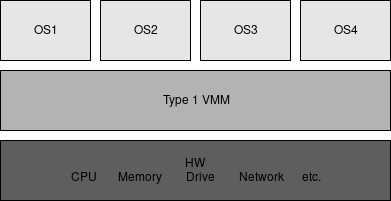
\includegraphics[width=0.65\textwidth]{png/VMMType1.png}
		\caption{Aufruf des FilterVIs}
		\label{fig:filterVI}
	\end{center}
\end{wrapfigure}
Ein Typ-1-Hypervisor (Bare-Metal oder auch native genannt) setzt direkt auf der Hardware auf. Es benötigt kein Betriebssystem, auf welchem dieses Läuft. Es wird jedoch vorausgesetzt, dass die Hardware des Host Systems vom Typ-1-Hypervisor durch entsprechende Treiber unterstützt wird.\\

\newpage
\subsubsection{Type 2}
\begin{wrapfigure}{r}{0.73\textwidth}
	\begin{center}
		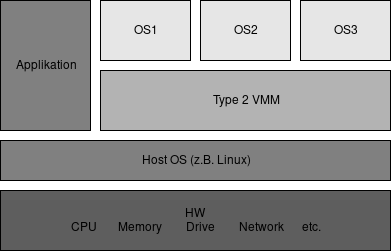
\includegraphics[width=0.6\textwidth]{png/VMMType2.png}
		\caption{Aufruf des asd}
		\label{fig:as}
	\end{center}
\end{wrapfigure}
Ein Typ-2-Hypervisor setzt auf einem vollwertigen Betriebssystem, welches auf dem Hostsystem installiert ist, auf und nutzt die Treiber, des Betriebssystems, um auf die Hardwareressourcen des Hostsystems zugreifen zu können. Dementsprechend sind alle Typ-2-Hypervisoren auf einem Hostsystem lauffähig, sofern sich auf diesem das unterstützte Host Betriebssystem installieren lässt.
\section{KVM}
KVM steht für Kernel Based Virtual Machine. bei KVM handelt es sich um eine Infrastruktur des Linux-Kernels zur Virtualisierung. Die Virtualisierung auf verschiedenen Plattformen unterstützt, unter anderem die folgenden Intel, AMD, ARM, PowerPC und System Z. KVM selbst nimmt keine Emulation vor, es ist also nicht möglich eine Bestimmte Hardware zu emulieren mit KVM selbst. so würde es sich als enorm Schwer erweisen ein vollwertiges Betriebssystem auf dem Hostsystem nur mit Hilfe von KVM zu installieren. Um die Emulation zu ermöglichen hat sich QEMU als de facto Standard etabliert. QEMU steht für Quick Emulator uns stellt für virtualisierte Gastsysteme die notwendigen Geräte wie Festplatten, Netzwerk-, Sound- und Grafikkarten zur Verfügung.\\
KVM ist desweiteren auch eine Quelloffene Lösung, und ist neben XEN der Weitverbreitete Quelloffene Hypervisor. Trotz einigen aussagen ist KVM jedoch ein Type 2 Hypervisor und nicht wie XEN ein Type 1.

\subsection{Funktionsumfang}
KVM ist bereits bei der Installation eine sehr schlanke und einfache Umgebung. 
Es sind im Wesentlichen nur die KVM Kernel Module dem bestehenden System zu installieren sowie Qemu und Management-Tools einzurichten. Der Vorteil liegt hier auch, dass viele schon bestehende Linux-Server nachträglich zu einem Virtualisierungssystem aufgerüstet werden kann ohne damit eine Komplette Neuinstallation tätigen zu müssen.
Weiter verhält sich jede  Virtuelle CPU (kurz VCPU) im Gastsystem wie ein gewöhnlicher Linux-Process und kann so beispielsweise auch über normale Kommandos wie kill oder top kontrolliert und gesteuert werden. Dasselbe gilt auch für die Gerätelandschaft. Da mit KVM und Qemu die normalen Linux-Treiber genutzt werden können, ist eine Umgewöhnung für einen Linux-Administrator nicht nötig.\\

KVM in Zusammenarbeit mit Qemu unterstützt eine enorme Anzahl an Gast-Betriebssysteme, darunter finden sich fast Sämtliche wichtigen Windows-Varianten sowie Linux, Solaris, BSD, FreeBSD und einige exotischere wie ReactOS.\\

Ein Nachteil der KVM ist jedoch, dass sie nicht auf Graphische Systeme ausgerichtet ist, es ist also die Idee, dass ein Gastsystem, welches auf einer KVM Instanz läuft, nur über ein Terminal bedient wird.\\
Beim Management zeigt sich, wie stark sich die Marktposition dieses Quelloffenen Open-Source-Hypervisors verbessert hat. Es ist inzwischen eine Fülle von Administrationswerkzeugen verfügbar, zudem wird KVM in vielen Cloud-Plattformen eingebaut.
Durch die simplen Tools virt-manager sowie virsh ist schon eine Remote-Management möglich. Für fortgeschrittene Funktionen wie Orchestrierung ganzer Pools von Virtuellen Maschinen mit weitergehenden Funktionen wie Failover, High Availability und dergleichen gibt es weitere Lösungen. Hier springen Dritt-Objekte sowie Softwarehersteller in die Bresche, normalerweise auch Open Source. 

Es gibt zudem für auf KVM aufbauende Komplettlösungen für die Servervirtualisierung. allen voran RHEV (Red Hat Virtualization).
Für die Verwaltung der Gastsysteme geben im Wesentlichen viele verschiedene Tools, von einfachen verwaltungssoftware für den Desktop PC wie zum Beispiel Gnome-Boxe

\newpage
\subsection{KVM on IBM z System}
KVM for IBM z Systems ist eine kostengünstige Alternative zu der von der IBM selbst entwickelten Virtualisierungslösung z/VM. KVM for IBM z System besitzt ein einfaches und gewohntes User-Interfaces, welche eine einfache Integration der z System Plattform in die IT Infrastruktur ermöglicht.
KVM for IBM z System ermöglicht zudem das den einzelnen Gastsystemen mehr Ressourcen zugeteilt wird, als das z System tatsächlich zur Verfügung stellt, dieser Umstand ermöglicht die optimale Auslastung der virtuellen Umgebung. Zusätzlich macht es die Plattform Mobilität einfacher und ist sogar in der Lage VMs und workloads zwischen verschiedenen Instanzen von KVM for IBM z System zu verschieben ohne dabei eine Ausfallzeit zu haben. \cite{website:ibm}
\begin{longtable}{|p{5cm}|p{10cm}|}
\hline
\textbf{Feature}                                     & \textbf{Benefit}                                                                                      \\ \hline
KVM Hypervisor                                       & Unterstützt das ausführen mehrere nicht gleicher Linux VMs auf einem einzelnen System.                  \\ \hline
CPU sharing                                          & Erlaubt es die Ressourcen der CPU über mehrere VMs hinweg zu teilen.                                   \\ \hline
I/O sharing                                          & Ermöglicht das teilen von I/O Ressourcen zwischen den VMs.                                             \\ \hline
Memory and CPU over-commitment                       & Erlaubt es einer VM mehr CPU, Memory und swapping space zu zuteilen als effektiv vorhanden ist.       \\ \hline
Live VM relocation                                   & Ermöglicht die Arbeitsbelastung zu migrieren mit minimalem Einfluss.                                  \\ \hline
Dynamic addition and deletion of virtual I/O devices & Reduziert Downtime um die I/O Geräte für die VMs zu konfigurieren.                                    \\ \hline
Thin-provisioned VMs                                 & Die VMDisk benötigt nur den belegten Speicherplatz, es wird so speicher gespart.                      \\ \hline
Hypervisor Performance Management                    & Unterstützung von policy-based, goal-oriented Management und Monitoring der virtuellen CPU Ressourcen. \\ \hline
Installation and Konfiguration Tools                 & Mitliefern von Tools um KVM for IBM z System zu installieren und Konfigurieren.                     \\ \hline
Transactional execution use                          & Bietet verbesserte Performance für das ausführen von multi-threaded Applikationen.                     \\ \hline
\end{longtable}
http://www.redbooks.ibm.com/redbooks/pdfs/sg248332.pdf

\subsubsection{Management Tools für KVM on IBM z System}
Dynamic Partition Manager kurz DPM.
DPM ist ein geführtes Management Interface im HMC (IBM Hardware Management Konsolen), mit welchem die z System Hardware und die virtuelle Infrastruktur mitsamt dem integriertem dynamischen I/O Management  definiert werden kann.\\
Unattended Installation (Unbeaufsichtigte Installation)
Unattended Installation des KVM Hypervisors vereinfacht die Administrations. Dies wird erreicht, indem ein Kickstart File erstellt wird, sowie dem hinzufügen des inst.auto=path\_to\_kickstart  Parameters im generic.prm File.

Single Hypervisor Management GUI
Kimchi ist ein OpenSource Management Tool, welches über ein intuitives Grafisches User Interface (GUI) für die folgende Management aufgaben verfügt.
\begin{itemize}
   \item Netzwerk Konfiguration für die OSA-based NICs
   \item Storage Konfiguration für ECKD und SCSI Geräte
   \item Standard System Informationen und Statistiken
   \item Debug Reports
   \item Hypervisor Neustart
\end{itemize}
\newpage
Enhanced Problem Determination Support
Viele verschiedene Tools wurden noch hinzugefügt um Probleme zu finden:
\begin{itemize}
   \item Ziorep -> eine Suite bestehend aus Tools, welche die SCSI Performance überwachen können.
   \item Das DASD dump Tool um einzelne DASD Geräte entleeren zu können.
   \item Das KDUMP Feature, welches Crash Dumps erstellt, falls ein Kernel Crash eintritt.
   \item dbginfo Skript, welches verschiedene system-related Files für Debug zwecke sammelt.
   \item Das sosreport Skript sammelt System fehlerbehebungs Informationen
\end{itemize}

\section{ESXi}
VMware ESXi (früher bekannt als ESX) ist ein Enterprise-Class, Typ-1 Hypervisor. Entwickelt wird dieser Typ-1 Hypervisor von VMware. Als ein Typ-1 Hypervisor, ist ESXI nicht eine Software Applikation, welche auf einem bestehenden Betriebssystem installiert wird, sondern, es beherbergt in sich schon wesentliche Komponente eines Betriebssystems, wie etwa den Kernel. \\

Nach der Version 4.1 benannte VMware ESX zu ESXi, ESXi ersetzte damals die Service Konsolen welches lediglich ein rudimentäres Betriebssystem war, mit einem besser integrierten Betriebssystem. ESX/ESXi ist die wichtigste Komponente der VMware Software Infrastruktur. \\

\subsection{Funktionsumfang}
Bei ESXi gibt es noch eine Sonderheit. ESXi ist zwar an sich kostenlos. So kann auf jedem Server / Rechner ESXi installiert werden ohne eine Lizenz bezahlen zu müssen. Möchte man jedoch ESXi auch verwalten und Konfigurieren so muss man sich den VMware vSphere hinzukaufen. Dies ist das Management Tool um den ESXi Hypervisor über die Distanz, also über das Lokale LAN zu konfigurieren. Dieses vSphere wird von VMware in 3 Lizenzversionen verkauft, welche über eine unterschiedliche Funktionspalette verfügt. Diese wurde nun in der Folgenden Tabelle dargelegt.

\begin{longtable}{|p{5cm}|p{3cm}|p{3cm}|p{3cm}|}
\hline
\textbf{Funktion und Merkmale}                                      & \textbf{Standard}                 & \textbf{Enterprise Plus}          & \textbf{Operations Management Enterprise Plus} \\ \hline
VMotion (Live-Migration)                                            & \checkmark                        & \checkmark                        & \checkmark \tabularnewline \hline
Storage VMotion (Live-Migration des Storages, z.B. in ein Cluster)  & \checkmark                        & \checkmark                        & \checkmark \tabularnewline \hline
Data Backupsolution                                                 & \checkmark                        & \checkmark                        & \checkmark \tabularnewline \hline
Fault Tolerance (Unterbrechungsfrei bei bis zu x VCPUs)             & 2 VCPUs                           & 4 VCPUs                           & 4 VCPUs    \tabularnewline \hline
Anti Virus System für alle VM (läuft nicht in den VMs)              & \checkmark                        & \checkmark                        & \checkmark \tabularnewline \hline
VSphere Replication (ermöglicht Replikation von Daten aus VM heraus)& \checkmark                        & \checkmark                        & \checkmark \tabularnewline \hline
VCenter HA                                                          & \checkmark                        & \checkmark                        & \checkmark \tabularnewline \hline
RecoverySolution                                                    & \checkmark                        & \checkmark                        & \checkmark \tabularnewline \hline
Verschlüsselung der VMs                                             &                                   & \checkmark                        & \checkmark \tabularnewline \hline
Virtuelle Laufwerke                                                 & \checkmark                        & \checkmark                        & \checkmark \tabularnewline \hline
Storage Policy-Based Management                                     & \checkmark                        & \checkmark                        & \checkmark \tabularnewline \hline
Distributed Resource \& Power Sheduler (Schaltet nicht gebrauchte VMS ab)&                               & \checkmark                        & \checkmark \tabularnewline \hline
Storage DRS (Speichert Daten der VMs so, dass Sie schneller gefunden werden)&                           & \checkmark                        & \checkmark \tabularnewline \hline
NVIDIA GRID vGPU                                                    &                                   & \checkmark                        & \checkmark \tabularnewline \hline
Flexible Operations Policies and Operations Groups                  &                                   &                                   & \checkmark \tabularnewline \hline
Role-based Access Control                                           &                                   &                                   & \checkmark \tabularnewline \hline
Scale-out Platform                                                  &                                   &                                   & \checkmark \tabularnewline \hline
\caption{Darstellung eines Kleinen Funktionsauszuges von \cite{website:vmwareEsxi}}
\end{longtable}

\chapter{Vergleich}
Um dem Vergleich einen fairen Tuch zu verleiten wurde hier Ausschliesslich KVM und ESXi miteinander verglichen und nicht KVM on IBM z System, da dieses Komplettpacket wohl für zwei total unterschiedliche einsatzgebiete gebraucht werden und dementsprechend kein guter vergleich zustande kommen könnte.

Es werden nur die Folgenden Punkte miteinander verglichen:
\begin{itemize}
	\item	Performance
	\item	Integration
	\item	Kosten
	\item	Komplexität
	\item	Maturity
	\item	Skalirbarkeit
	\item	Funktionssupport
\end{itemize}

\subsubsection{Performance}

Hypervisoren sind in zwei unterschiedlichen Typen unterteilt, welche einen Einfluss auf die Performance haben. Type 1 Hypervisoren, welche auch bekannt als "Bare-Metal" sind, laufen direkt auf der physikalischen Hardware, und das Betriebssystem jedes Gastsystemes läuft auf dem Hypervisor. Diese Hypervisoren erlauben normalerweise einigen Gästen den Hypervisor zu Kontrollieren. Viele Unternehmen setzen auf den Typ 1 Hypervisor.

Ein Typ 2 Hypervisor, auch bekannt als hosted Hypervisor, läuft in einem Betriebssystem, welches wiederum auf einer Physikalischen Hardware läuft. Das Gastsystem läuft anschliessend auf dem Hostsystem. Desktop Hypervisoren sind meistens Typ 2 Hypervisors.

Das beste Beispiel für einen puren Typ-1 Hypervisor ist XEN, jedoch auch ESXi, welches definitiv auch ein Type-1 Hypervisor ist, da es keine Applikation ist, welche auf einem Betriebssystem installiert wird. ESXi besteht aus einem Kernel und weiteren OS Komponenten, welche es ins eigene native OS integriert hat.

Die Klassifikation von KVM stellt ein etwas grösseres Problem dar. Der Grund für die Schwierigkeiten ist, dass KVM eigenschafte beider Hypervisor Typen beinhaltet. Es wird als eine Linux Komponente vertrieben. Dies bedeutet, dass ein Linux User KVM von der Command Line oder per GUI starten kann. Das KVM so gestartet werden kann lässt es so aussehen, als sei es eine Applikation, welche auf einem Betriebssystem läuft, obschon KVM im Kernel integriert ist und dadurch auch direkt auf der Maschine Läuft.
Das Host Betriebssystem stellt KVM ein Start Mechanismus, nach welchem es eine Co-Processing Beziehung mit ihm aufbaut. Diese Co-Processing Beziehung erlaubt es KVM die physische Hardware direkt zu Kontrollieren. KVM macht von den Prozessor Virtualisierung Instruktionen auf der x86 Hardware gebrauch. Dies erlaubt es dem Hypervisor und all seinen Gästen direkt auf der Hardware zu laufen, also Bare-Metal. Die physikalische Hardware für die meisten Resource Translation aus, so das KVM die traditionellen Kriterien für einen Typ 1 Hypervisor erfüllen würde und dennoch wird es als ein Typ 2 Hypervisor eingestuft.

Auch wenn bekanntermassen ein Typ 1 Hypervisor schneller laufen sollte als ein Typ2 so ist dies bei KVM und ESXi nicht der Fall. KVM kann hier mit einer besseren Startzeit punkten und auch einer etwas besseren Performance, was sich jedoch bei einem normalen Workload kaum unterscheiden lässt.

\subsubsection{Integration}
Die verschiedenen Hypervisoren nutzten auch verschiedene Methoden um mit der physikalischen Hardware des Hosts zu Kommunizieren. KVM benutzt dazu einen Agent, welcher auf dem Host installiert ist um mit der Hardware zu Kommunizieren, ESXi hingegen nutzt VMware Management plane um mit der Hardware zu kommunizieren. VMware's Lösung ermöglicht es ESXi auf anderen VMware Produkte, welche auch die Management plane nutzten, zuzugreifen. Dies erfordert jedoch auch, dass ESXi VMware control stack verwenden muss, was zu einer erhöhten Hardware Requirement führt.

Starke Integration mit dem Host OS ist normalerweise der primäre Grund, weshalb Linux Entwickler KVM bevorzugen. Da KVM kurz nach dessen Release in den Linux Kernel integriert wurde. Zum Vergleich, Xen wurde nicht offiziell in den Kernel integriert bis 2011, also 8 Jahre nach dessen Einführung. Zudem wird es bevorzugt, da viele Linux distributionen KVM als präferierten Hypervisor adaptiert haben.

\subsubsection{Kosten}

KVM gewinnt klar gegen VMware wenn es zu den Kosten kommt. KVM ist OpenSource, dies bedeutet, dass keine weiteren Kosten für den Endbenutzer anfallen. Es wird oft auf verschiedenen Wegen vertrieben, meist als ein Teil einer open Source Lösung.

VMware charges a license fee to use its products, including ESXi. It’s able to do this because VMware was the first company to release enterprise-class virtualization software and is still the market leader in this segment. Its brand is therefore still relevant to an business’s end users, regardless of what developers may think about it. An ESXi user must also purchase a license to use vSphere, VMware’s suite of tools for cloud computing that uses ESXi. Additional software licenses may be needed, which will further increase the cost of implementing ESXi.

IBM performed some calculations regarding the total cost of ownership (TCO) for KVM and VMware in 2012. These calculations showed the KVM’s TCO was typically 39 percent less than VMware, although the actual TCO will depend on site-specific factors such as the operational setting and workload. This difference in TCO indicates that cloud service providers will probably want to implement KVM on at least one cluster, regardless of the other factors to consider.
\subsubsection{Complexity}

A comparison of KVM and VMware also show a clear difference in the size of the code base, which affects a hypervisor’s maintenance costs. KVM was initially released to take advantage of processor extensions that allowed them to virtualize guests without translating binary code. This origin meant that the first stable release of KVM was essentially a lightweight virtualization driver, with little more than 10,000 lines of code (LOC).

VMware is believed to have over 6 million LOC, although this fact can’t be verified since its source code isn’t publicly available. This total doesn’t directly affect performance since VMware uses hardware extensions to virtualize guest. Nevertheless, its original code has never been completely rewritten, resulting in a more complex code base than KVM.
\subsubsection{Maturity}

KVM and ESXi are both highly mature and stable. KVM has been part of the Linux kernel for over a decade, and ESXi has been publicly available since 2006. However, KVM is more widely deployed since it’s open source and is included in many packages such as Redhat Enterprise Virtualization (RHEV). KVM also supports more features than any other hypervisor.
\subsubsection{Scalability}

KVM is generally more scalable than VMware, primarily because vSphere has some limitations on the servers it can manage. Furthermore, VMware has added a large number of Storage Area Networks (SANs) to support various vendors. This feature means that VMware has more storage options than KVM, but it also complicates VMware’s storage support when scaling up.
\subsubsection{Functionality Support}

Hypervisors vary greatly in their support of functionality. Network and storage support are especially important and are probably more important than any other factor besides OS integration. It shouldn’t come as a surprise to learn that ESXi’s support for other VMware products is unmatched by any other hypervisor. On the other hand, KVM offers more options for network support than VMware.

\chapter{Fazit}
KVM is typically the most popular choice for users who are concerned about the cost of operating each VM and less interested in enterprise-level features. This rule primarily applies to providers of cloud and host services, who are particularly sensitive to the cost and density of their servers. These users are highly likely to choose open-source hypervisors, especially KVM.

The tight integration with the host OS is one of the most common reasons for developers to choose KVM, especially those who use Linux. The inclusion of KVM in many Linux distributions also makes it a convenient choice for developers. KVM is also more popular among users who are unconcerned about brand names.
\chapter{Anhang}
\printbibliography

https://www.cs.hs-rm.de/~linn/fachsem0910/hirt/KVM.pdf
https://www.tecchannel.de/a/kostenlose-virtualisierungssoftware-im-vergleich,2051909,4
https://www.tecchannel.de/a/kostenlose-virtualisierungssoftware-im-vergleich,2051909,5
https://www.rippleweb.com/vmware-vs-kvm/
\end{document}

